%\documentclass[a4paper,9pt,fleqn,notoc]{diss}
%\renewcommand{\includegraphics}[1][1]{} 

%\begin{document}

%%%%%%%%%%%%%%%%%%%%%%%%%%%%%%%%%%%%
\chapter{German locative phrases -- an introduction}
\label{s:german-spatial-language-introduction}
%syntactic distinctions mirror semantic distinctions\\
%vast space of semantic distinctions or spatial conceptualizations\\
%vast space of possible syntactic expression of spatial conceptualzations\\

To appreciate the complexity of spatial language one just needs
to consider a particular human language such as German.
The following chapters detail an elaborate reconstruction 
effort which targets locative German phrases (parts of this reconstruction
effort have been published in \citealt{spranger2011german}\oldindex{Loetzsch, M.}\oldindex{Spranger, M.}). 
I specifically focus on the processing of German locative phrases 
in a whole systems approach encompassing the perception, conceptualization,
as well as production and parsing of spatial phrases.
Before we jump to the implementation and the specific
challenges in modeling such a complex phenomenon, this introduction
overviews German spatial relations and highlights the syntax and 
semantics of German locative phrases, as well as the
close interaction of syntax and semantics. 
The claim is that important aspects of the syntactic structure of an utterance, i.e. 
the lexical items and the grammatical relations between them, work together to convey 
semantic structure, i.e. meaning. Vice versa, the varied syntactic 
devices in German spatial language allow to express subtle differences
in the conceptualization of spatial scenes. The German spatial language system serves 
as a beautiful example of how syntax connects to the extraordinarily rich world of 
spatial semantics. %The following paragraphs give a quick introduction to 
%German locative expressions. % We know this already.

%%%%%%%%%%%%%%%%%%%%%%%%%%%%%%%%%%%%

%\paragraph*{Spatial Relations}
% projective, topological
The literature distinguishes several classes of spatial relations 
available in German. Among them are projective, proximal and absolute relations
(see \figref{f:spatial-relations-taxonomy}).
\begin{description}
\item[Projective relations]\is{spatial relation!projective}-- sometimes also called \textsc{dimensional terms} 
\citep{eschenbach2004functional,herskovits1986language}\oldindex{Eschenbach, C.}\oldindex{Herskovits, A.} --  
in German comprise the class of six items referring to spatial dimensions
\textit{vor} (`front'), hinter (`behind'), \textit{\"uber} (`above'), \textit{unter} (`below'), \textit{rechts} (`right'), 
\textit{links} (`left') \citep{tenbrink2007space,tenbrink2005localising,wunderlich1991lokale}\oldindex{Herweg, M.}\oldindex{Tenbrink, T.}\oldindex{Wunderlich, D.}. 
Traditionally, and for reasons of distinct syntax and semantics the
class of projective relations is further divided into \textsc{frontal} (\textit{vor} 
and \textit{hinter}), \textsc{lateral} (\textit{links} and \textit{rechts}), 
\textsc{horizontal} (comprising lateral and frontal relations), and 
\textsc{vertical relations} (\textit{\"uber} and \textit{unter}). 
\item[Proximal relations] are part of the larger class of topological relations\is{spatial relation!proximal}
that structure space with respect to proximity, contact and inclusion 
\citep{Grabowski1996prepositional}\oldindex{Weiss, P.}\oldindex{Grabowski, J.}. For this book proximal relationships
such as \textit{nah} (`near') and \textit{fern} (`far') are important.
\item[Absolute relations] refer to cardinal directions,\is{spatial relation!absolute}
for instance \textit{n\"ordlich} (`north'), \textit{westlich} (`west'), \textit{\"ostlich} (`east') and
\textit{s\"udlich} (`south').
\end{description}

\begin{sidewaysfigure}
%\begin{figure}
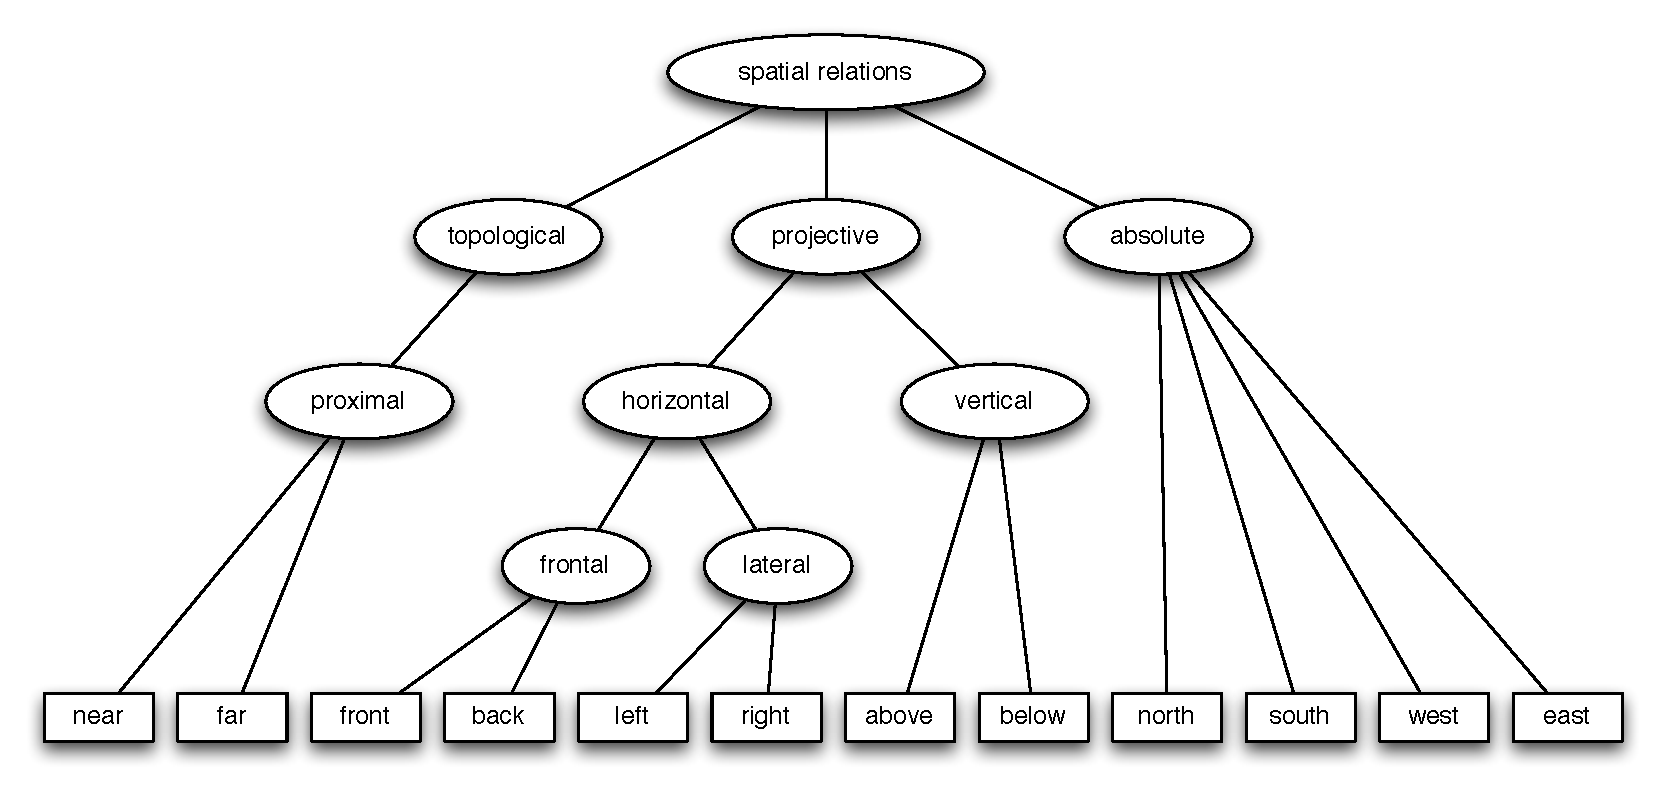
\includegraphics[width=\columnwidth]{figs/spatial-relations-taxonomy}
\label{f:spatial-relations-taxonomy}
\caption[Taxonomy of spatial relations in German.]{%
Taxonomy of spatial relations discussed in this book.
The rectangular items refer to the spatial terms used for denoting
the relations. Since in German spatial relations can be expressed in
different lexical classes and word forms, English
equivalents are used as placeholder.}
%\end{figure}
\end{sidewaysfigure}

Spatial relations take different syntactic forms in German. 
All of the projective terms, for instance, can be expressed in different 
lexical classes, most prominently as adjectives, adverbs and prepositions. 
For example, the projective term \textit{vor} can appear as adjective as in 
\REF{e:5:der-vordere-block}, as adverb as in \REF{e:5:der-block-vorne} 
and as preposition as in \REF{e:5:der-block-vor-der-kiste}. 
\is{adjectives}
\ea
\label{e:5:der-vordere-block}
\gll der vordere Block\\
the.{\NOM} front.{\ADJ}.{\NOM} block.{\NOM} \\
\glt `The front block'\\
%\glend
\z
\ea
\label{e:5:der-block-vorne}
\gll der Block vorne\\
the block.{\NOM} {in the front.{\ADV}} \\
\glt `The front block'\\
%\glend
\z
\ea
\label{e:5:der-block-vor-der-kiste}
\gll der Block vor der Kiste\\
the.{\NOM} block.{\NOM} front.{\PREP} the.{\DAT} box.{\DAT} \\
\glt `The block in front of the box.'\\
%\glend
\z

The different lexical classes carry with them different 
syntactic functions, e.g. adjectives can function as modifiers
in determined adjective noun phrases, prepositions are followed
by noun phrases and in German govern case.  
But each lexical class is also connected 
to a different semantic interpretation. In particular, there is 
a tight connection between the lexical class and specific spatial 
construal operations that govern how precisely the spatial relation is
to be applied. The meaning
of a projective category when used as an adjective is to filter objects 
\citep{tenbrink2007space}\oldindex{Tenbrink, T.}, whereas when used as preposition the 
meaning is to construct a region \citep{klabunde1999logic}\oldindex{Klabunde, R.}. 
For instance, the following phrase \REF{e:5:stelle-den-stuhl-vor-den-schrank} uses the projective category
front to construct a region to which one is asked to put a chair. 
Unlike in the adjective case, the region is not used to modify
or filter, rather the region is necessarily empty in order for the chair to be put there. 

\ea
\label{e:5:stelle-den-stuhl-vor-den-schrank}
\gll Stelle den Stuhl vor den Schrank!\\
Put the chair front.{\PREP} the cupboard\\
\glt `Put the chair in front of the cupboard!'\\
%\glend
\z

%%%%%%%%%%%%%%%%%%%%%%%%%%%%%%%%%%%%
%\paragraph*{Prepositions}
Another important difference between spatial adjectives and spatial adverbs and prepositions is the potential
for \textsc{reference objects} or \textsc{landmarks}. Example 
\REF{e:5:der-block-vor-der-kiste} relates a \textsc{located object}, also called
``figure'' \citep{talmy2000toward2}\oldindex{Talmy, L.} and ``trajector'' \citep{vandeloise1991spatial}\oldindex{Vandeloise, C.}
to a reference object, also called ``landmark'' \citep{vandeloise1991spatial}\oldindex{Vandeloise, C.}, 
``relatum'' \citep{tenbrink2007space}\oldindex{Tenbrink, T.} or ``ground'' \citep{talmy2000toward2}\oldindex{Talmy, L.}.
If a spatial term is used prepositionally as in 
\REF{e:5:der-block-vor-der-kiste}, both the spatial relation, in this case 
\textit{vor}, and the landmark \textit{Kiste} (`box'), are expressed in the 
prepositional phrase itself. \is{prepositions}

%%%%%%%%%%%%%%%%%%%%%%%%%%%%%%%%%%%%
%\paragraph*{Adverbs}
A third possible lexical class, in which spatial relations partake, are adverbs. \is{adverbs}
Spatial adverbs can be accompanied
by a prepositional phrase, as in \REF{e:5:der-block-vorne-in-der-kiste}--\REF{e:5:der-block-links-von-der-kiste}:
\ea
\label{e:5:der-block-vorne-in-der-kiste}
\gll der Block vorne in der Kiste\\
the.{\NOM} block.{\NOM} front.{\ADV} of.{\PREP} the.{\DAT} box.{\DAT}\\
\glt `The block in the front of the box'\\
%\glend
\z
\ea
\label{e:5:der-block-links-von-der-kiste}
\gll der Block links von der Kiste\\
the.{\NOM} block.{\NOM} left.{\ADV} of.{\PREP} the.{\DAT} box.{\DAT}\\
\glt `The block to the left of the box'\\
%\glend
\z
The prepositional phrases \textit{in der Kiste} and \textit{von der Kiste}  both introduce
a landmark which, via
the spatial term, relates to the figure, in this case \textit{der Block}. The two different prepositions \textit{in} and \textit{von}
denote whether the relation referred to by the spatial term is \textsc{internal} 
to the landmark or \textsc{external}. In the case of \textit{von}, the spatial
region denoted by the projective adverb, e.g. \textit{links} (`left'), is external to the 
landmark, whereas in the case of \textit{in} the region lies within the landmark. 
The projective 
adverbs \textit{links} (`left') and \textit{rechts} (`right') can be followed both by 
\textit{von} and \textit{in} prepositional phrases, hence they can have an internal
and external reading. The projective adverbs \textit{vorne} (`front') 
and \textit{hinten} (`back') can only be extended by \textit{in} prepositional phrases. 
The vertical projective adverbs \textit{oben} (`above') and \textit{unten} (`below')
elicit internal readings. Again differences in semantic processing are 
syntactically marked, in the case of adverbs by prepositional phrases
that complement the adverb.

%\begin{figure}
%\label{f:region-external-vs-internal}
%\caption[Internal vs external regions.]{TODO: figure}
%\end{figure}

%%%%%%%%%%%%%%%%%%%%%%%%%%%%%%%%%%%%
%\paragraph*{Perspective Marking}
The last important component of spatial language considered in this book
is perspective marking. The following two example feature perspective markers. In \REF{e:5:der-block-vorne-von-dir-aus} an adverb is perspective marked, in \REF{e:5:der-block-links-der-kiste-von-dir-aus} a prepositional
phrase is perspective marked.
\ea
\label{e:5:der-block-vorne-von-dir-aus}
\gll der Block vorne von dir aus\\
the.{\NOM} block.{\NOM} front.{\ADV} from.{\PREP} the.{\DAT} box.{\DAT} \\
\glt `The block in front from your perspective'\\
%\glend
\z
\ea
\label{e:5:der-block-links-der-kiste-von-dir-aus}
\gll der Block links der Kiste von dir aus\\
the.{\NOM} block.{\NOM} left.{\PREP} the.{\GEN} box.{\GEN} from.{\PREP} your.{\DAT} perspective\\
\glt `The block to the left of the box from your perspective'\\
%\glend
\z
Perspective on a scene is important for particular interpretations
of spatial phrases, because it influences how the spatial scene and in 
particular the landmark is conceptualized. 


%\paragraph*{}

%\section{A Whole Systems Approach to German Spatial Language}
These few examples from German locative phrases show that 
we can analyze the syntax of spatial language 
fruitfully in terms of its spatial semantics. This resonates with 
theories of syntax which put the direct
mapping of syntax to semantics at the core of language processing, such as Construction Grammar.
The tight relationship between syntax and semantics is an important 
claim in this book which underlies the reconstruction efforts, and also
the evolution experiments. 

The first question I am focusing on is how to organize language processing.
That is, how semantics is encoded in words and grammar -- and vice versa.
However, this is not the full story. One needs to ground language in 
perception. Speakers need to be able to plan what they are going 
to say based on their communicative intention. Hearers must have machinery for
interpreting the utterance based on the spatial context. This widens the question
from how to organize the syntax and semantics interface to how to organize 
processing in a large array of systems comprising perception, conceptualization,
interpretation and also processing of syntax. In particular,
one has to identify the cognitive operations underlying the semantics of
German locative phrases and how these operations are used in conceptualization
of spatial scenes, as well as how conceptualization interacts with the
perception of spatial scenes.  The following section examine three main questions. 
First, what is the meaning of phrases such as
\textit{der Block links von der Box von dir aus} (`the block left of the box from your 
perspective', see \REF{e:5:der-block-links-der-kiste-von-dir-aus}) and
how can we formalize the semantic structure of these utterances?
What are the cognitive primitives that are necessary for modeling the 
semantics of spatial phrases in particular? Second, how does semantic structure get translated into 
words and grammatical relations and back? And thirdly how can agents 
autonomously conceptualize spatial scenes given
communicative goals and how can agents interpret semantic structure recovered in parsing
so that success in communication can be achieved?

%\bibliographystyle{diss}
%\bibliography{papers,space} 
%\end{document}
